\documentclass[10pt,aspectratio=1610]{beamer}
\usetheme[
%%% options passed to the outer theme
%    hidetitle,           % hide the (short) title in the sidebar
%    hideauthor,          % hide the (short) author in the sidebar
%    hideinstitute,       % hide the (short) institute in the bottom of the sidebar
%    shownavsym,          % show the navigation symbols
%    width=2cm,           % width of the sidebar (default is 2 cm)
%    hideothersubsections,% hide all subsections but the subsections in the current section
%    hideallsubsections,  % hide all subsections
%    left                % right of left position of sidebar (default is right)
  ]{Aalborg}
  
\definecolor{orangeUGR}{RGB}{254,55,11}
\definecolor{greyUGR}{RGB}{125,126,126}
% If you want to change the colors of the various elements in the theme, edit and uncomment the following lines
% Change the bar and sidebar colors:
\setbeamercolor{Aalborg}{fg=black!20,bg=greyUGR}
%\setbeamercolor{sidebar}{bg=greyUGR!20}
% Change the color of the structural elements:
\setbeamercolor{structure}{fg=black}
% Change the frame title text color:
\setbeamercolor{titlepagecolorbox}{fg=greyUGR,bg=greyUGR!20}
\setbeamercolor{frametitle}{fg=orangeUGR}
\setbeamercolor{subtitle}{fg=orangeUGR}
\setbeamercolor{section in sidebar}{fg=orangeUGR}
% Change the normal text color background:
%\setbeamercolor{normal text}{bg=gray!10}
% ... and you can of course change a lot more - see the beamer user manual.
\usepackage{xcolor}
\usepackage[utf8]{inputenc}
\usepackage[english]{babel}
\usepackage[T1]{fontenc}

% Or whatever. Note that the encoding and the font should match. If T1
% does not look nice, try deleting the line with the fontenc.
\usepackage{helvet}


% colored hyperlinks
\newcommand{\chref}[2]{%
  \href{#1}{{\usebeamercolor[bg]{Aalborg}#2}}%
}



\title[Gated Sensor Fusion for Human Body Motion Estimation]% optional, use only with long paper titles
{Gated Sensor Fusion: A way to Improve the Precision of Ambulatory Human Body Motion Estimation}

\subtitle{KES Innovation in Medicine and Healthcare InMed-14}  % could also be a conference name

\date{July 9, 2014}

\author[A. Olivares et al.]{Alberto Olivares\inst{1} \and Juan Manuel G\'orriz\inst{1} \and Javier Ram\'irez\inst{1} \and Gonzalo Olivares\inst{2}}

\institute[Universidad de Granada] % (optional)
{
  \inst{1}%
  Dept. of Signal Theory, Networking and Communications, Universidad de Granada, Spain
  \and
  \inst{2}%
  Detp. of Computer Architecture and Computer Technology, Universidad de Granada, Spain
}

% specify the logo in the top right/left of the slide
\pgfdeclareimage[height=1cm]{mainlogo}{AAUgraphics/escudougr.eps} % placed in the upper left/right corner
\logo{\pgfuseimage{mainlogo}}

% specify a logo on the titlepage (you can specify additional logos an include them in 
% institute command below
\pgfdeclareimage[height=1.5cm]{titlepagelogo}{AAUgraphics/logoalter.eps} % placed on the title page
%\pgfdeclareimage[height=1.5cm]{titlepagelogo2}{AAUgraphics/aau_logo_new} % placed on the title page
\titlegraphic{% is placed on the bottom of the title page
  \pgfuseimage{titlepagelogo}
%  \hspace{1cm}\pgfuseimage{titlepagelogo2}
}

\begin{document}
%%%%%%%%%%%%%%%%%%%%%%%%%%%%%%%%%%%%%%%%%%%%%%%%
{\aauwavesbg
\begin{frame}[plain,noframenumbering] % the plain option removes the sidebar and header from the title page
  \titlepage
\end{frame}}
%%%%%%%%%%%%%%%%%%%%%%%%%%%%%%%%%%%%%%%%%%%%%%%%


%%%%%%%%%%%%%%%%%%%%%%%%%%%%%%%%%%%%%%%%%%%%%%%%
\begin{frame}{Outline}{}
\tableofcontents
\end{frame}
%%%%%%%%%%%%%%%%%%%%%%%%%%%%%%%%%%%%%%%%%%%%%%%%


%%%%%%%%%%%%%%%%%%%%%%%%%%%%%%%%%%%%%%%%%%%%%%%%
\section{Introduction}
\label{sec:introduction}
\begin{frame}{Introduction}{}

\begin{block}{Measuring human motion  in medical practice}
\begin{columns}
\begin{column}{.5\textwidth}
 \begin{itemize}
  \item Helps physicians to assess patients:
  \begin{itemize}
  	\item With neurodegenerative diseases.
  	\item Following rehabilitation processes.
  	\item In risk of falling. 
  	\item With gait disorders.
  	\item With sleep disorders.
  	\item Suffering unnoticed nocturnal epileptic seizures.
  \end{itemize}
  \end{itemize} 
\end{column}
\begin{column}{.5\textwidth}
\centering
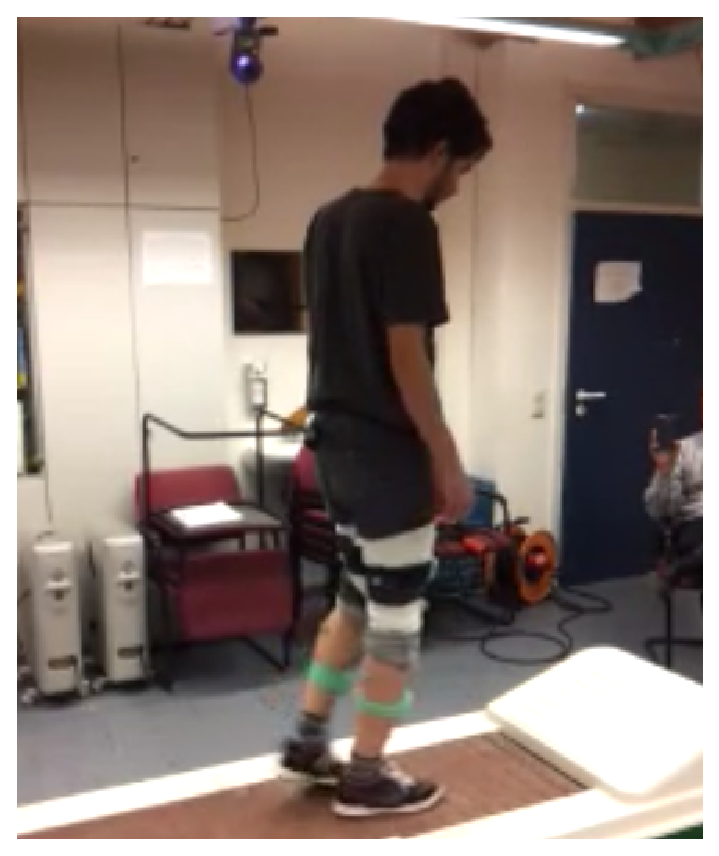
\includegraphics[width=0.4\textwidth]{AAUgraphics/subject.eps}
\end{column} 

\end{columns}
\end{block}
\end{frame}
%%%%%%%%%%%%%%%%%%%%%%%%%%%%%%%%%%%%%%%%%%%%%%%%


%%%%%%%%%%%%%%%%%%%%%%%%%%%%%%%%%%%%%%%%%%%%%%%%
\begin{frame}{Introduction}{}

\begin{block}{Human motion can be measured in different ways}
\begin{columns}
    \begin{column}{.5\linewidth}
	    \begin{itemize}
	    	\item Camera-based systems
	    	\begin{itemize}
	    		\item Cameras acting as observers.
	    		\item Very accurate.
	    		\item Reduced flexibility.
	    		\item Reduced range (non ambulatory).
	    		\item Expensive.
	    		\item Privacy issues.
	    		\item Examples: \textit{Vicon},\textit{Qualisys}.
	    	\end{itemize}
	    \end{itemize}
	    \vspace{0.6cm}
	    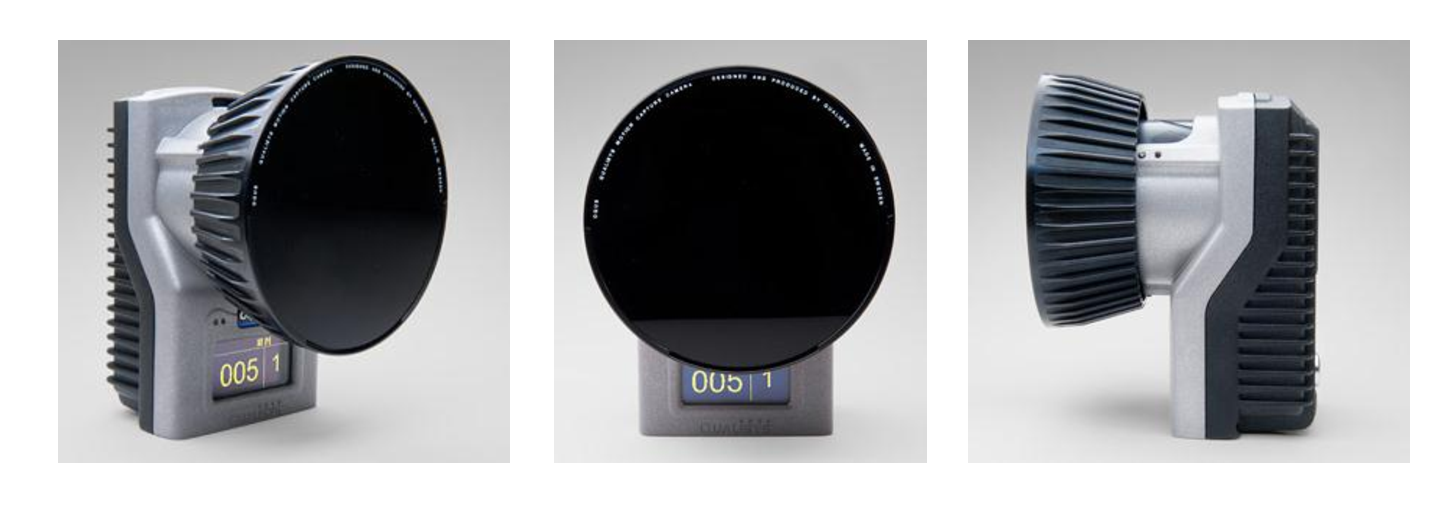
\includegraphics[width=1\textwidth]{AAUgraphics/bla.eps}	
	    \vspace{0.3cm}
    \end{column}
    	     
    \begin{column}{.5\linewidth}
    	\begin{itemize}
	    	\item Inertial systems
	    	\begin{itemize}
	    		\item Inertial sensors in IMUs.
	    		\item Lower accuracy.
	    		\item High flexibility.
	    		\item Ambulatory.
	    		\item Non-expensive.
	    		\item No privacy issues.
	    		\item Examples: \textit{Xsens}, \textit{Shimmer}.
	    	\end{itemize}
    	\end{itemize}
    	 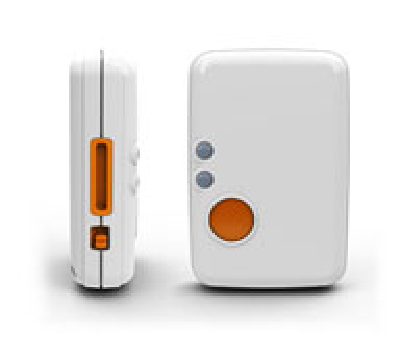
\includegraphics[width=0.5\textwidth]{AAUgraphics/Shimmer.eps}
    	 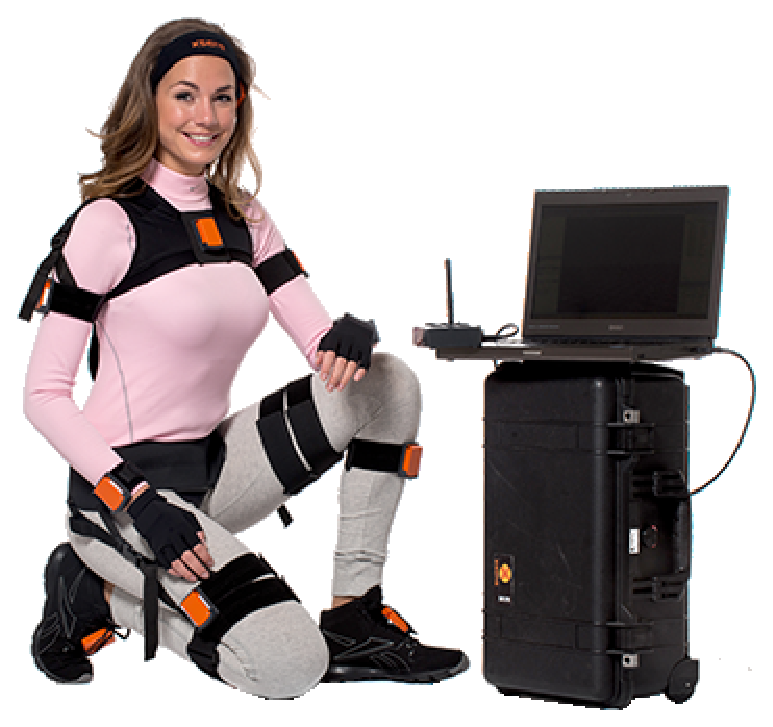
\includegraphics[width=0.5\textwidth]{AAUgraphics/xsens.eps}    
    \end{column}
\end{columns}
\end{block}
\end{frame}
%%%%%%%%%%%%%%%%%%%%%%%%%%%%%%%%%%%%%%%%%%%%%%%%

%%%%%%%%%%%%%%%%%%%%%%%%%%%%%%%%%%%%%%%%%%%%%%%%
\begin{frame}{Introduction}{}
\begin{block}{Orientation estimation algorithms have constant parameters}
\begin{itemize}
	\item Kalman filters performance highly dependent on constant parameters.
	\item Parameters control confidence balance between estimation and observation.
	\item Observation: orientation estimation using accelerometer.
	\item Observation only reliable when motion intensity is low.
	\item High motion intensity $\rightarrow$ High linear acceleration.
	\item Non satisfactory precision under changing motion conditions.
	\item Optimal value of parameters different for low and high intensity.
\end{itemize}
\end{block}
\begin{block}{We propose}
\begin{itemize}
	\item Dynamical modification of static parameters.
	\item Optimal values are switched according to detected motion intensity.
	\item Intensity is detected using spectrum analysis of acceleration signals.
\end{itemize}
\end{block}
\end{frame}
%%%%%%%%%%%%%%%%%%%%%%%%%%%%%%%%%%%%%%%%%%%%%%%%

%%%%%%%%%%%%%%%%%%%%%%%%%%%%%%%%%%%%%%%%%%%%%%%%
\section{Previous Work}
\label{sec:previous_work}
\subsection{Orientation Estimation}
\label{subsec:orientation_estimation}
\begin{frame}{Previous Work}{Orientation Estimation}
\begin{block}{Developed in the 70s for space missions}
	\begin{itemize}
		\item To determine orientation of the spaceship.
		\item Examples: TRIAD and QUEST.
		\begin{itemize}
			\item Orientation of two vector observations with respect to two vector references.
			\item Vector observations: Magnetic field and acceleration in body frame.
			\item Vector references: Local Gravity and Earth magnetic field vectors.
			\item Only acceleration and magnetic field.
			\item Output: orientation quaternion.
		\end{itemize}
	\end{itemize}	
\end{block}
\begin{block}{Recent approaches}
\begin{itemize}
	\item Fuse estimated quaternion with angular velocity orientation quaternion.
	\item Estimate orientation quaternion in different ways.
	\item Many variations have been proposed ALL with permanent tunning parameters.
\end{itemize}
\end{block}
\end{frame}
%%%%%%%%%%%%%%%%%%%%%%%%%%%%%%%%%%%%%%%%%%%%%%%%


%%%%%%%%%%%%%%%%%%%%%%%%%%%%%%%%%%%%%%%%%%%%%%%%
\section{Theoretical Background}
\label{sec:theory}
\subsection{Intensity Detectors}
\label{subsec:intensity_detectors}
\begin{frame}{Theoretical Background}{Intensity Detectors}
\begin{block}{We need to estimate motion intensity}
\begin{itemize}
	\item There are many possibilities.
	\item Time analysis of acceleration and/or angular velocity.
	\begin{itemize}
		\item Magnitude. 
		\item Variance.
	\end{itemize}
	\item Frequency analysis of acceleration and/or angular velocity.
	\begin{itemize}
		\item Framed Spectrum.
		\item Long Term Spectral Envelope.
		\item Estimation of PSDs.
	\end{itemize}
	\item Output is compared to a predefined threshold to create a binary marker.
	\item Binary marker: 1 (high intensity), 0 (low intensity).
\end{itemize}
\end{block}
\end{frame}
%%%%%%%%%%%%%%%%%%%%%%%%%%%%%%%%%%%%%%%%%%%%%%%%


%%%%%%%%%%%%%%%%%%%%%%%%%%%%%%%%%%%%%%%%%%%%%%%%
\begin{frame}{Theoretical Background}{Intensity Detectors}
\begin{block}{In this work we used}
\begin{itemize}
	\item The Framed Spectrum Detector $\rightarrow$ computationally efficient and accurate.
	\item Input $\rightarrow$ Acceleration magnitude.
	\item Output:
\end{itemize}
\begin{columns}
	\begin{column}{.5\linewidth}
		\small
		\begin{equation}
		\mbox{V}(\mathbf{n})=10\log_{10}\left(\frac{1}{\mbox{N}_{\scriptsize 	\mbox{FFT}}}\sum_{l=0}^{\mbox{N}_{\scriptsize \mbox{FFT}}-1}\frac{\mbox{X}^{2}(l,n)}{\mbox{N}^{2}(l)}\right)
		\label{eq:fsd}
		\nonumber
		\end{equation}
		\normalsize
		\begin{itemize}
			\item $\mbox{N}_{\scriptsize \mbox{FFT}}$ resolution of the FFT.
			\item N($l$): Average noise spectrum magnitude for the $l$ band.
			\item $\mbox{X}(l,n)$ spectrum of input signal for the $l$ band at frame $n$.
		\end{itemize}
	\end{column}
	\begin{column}{.5\linewidth}
		\centering
		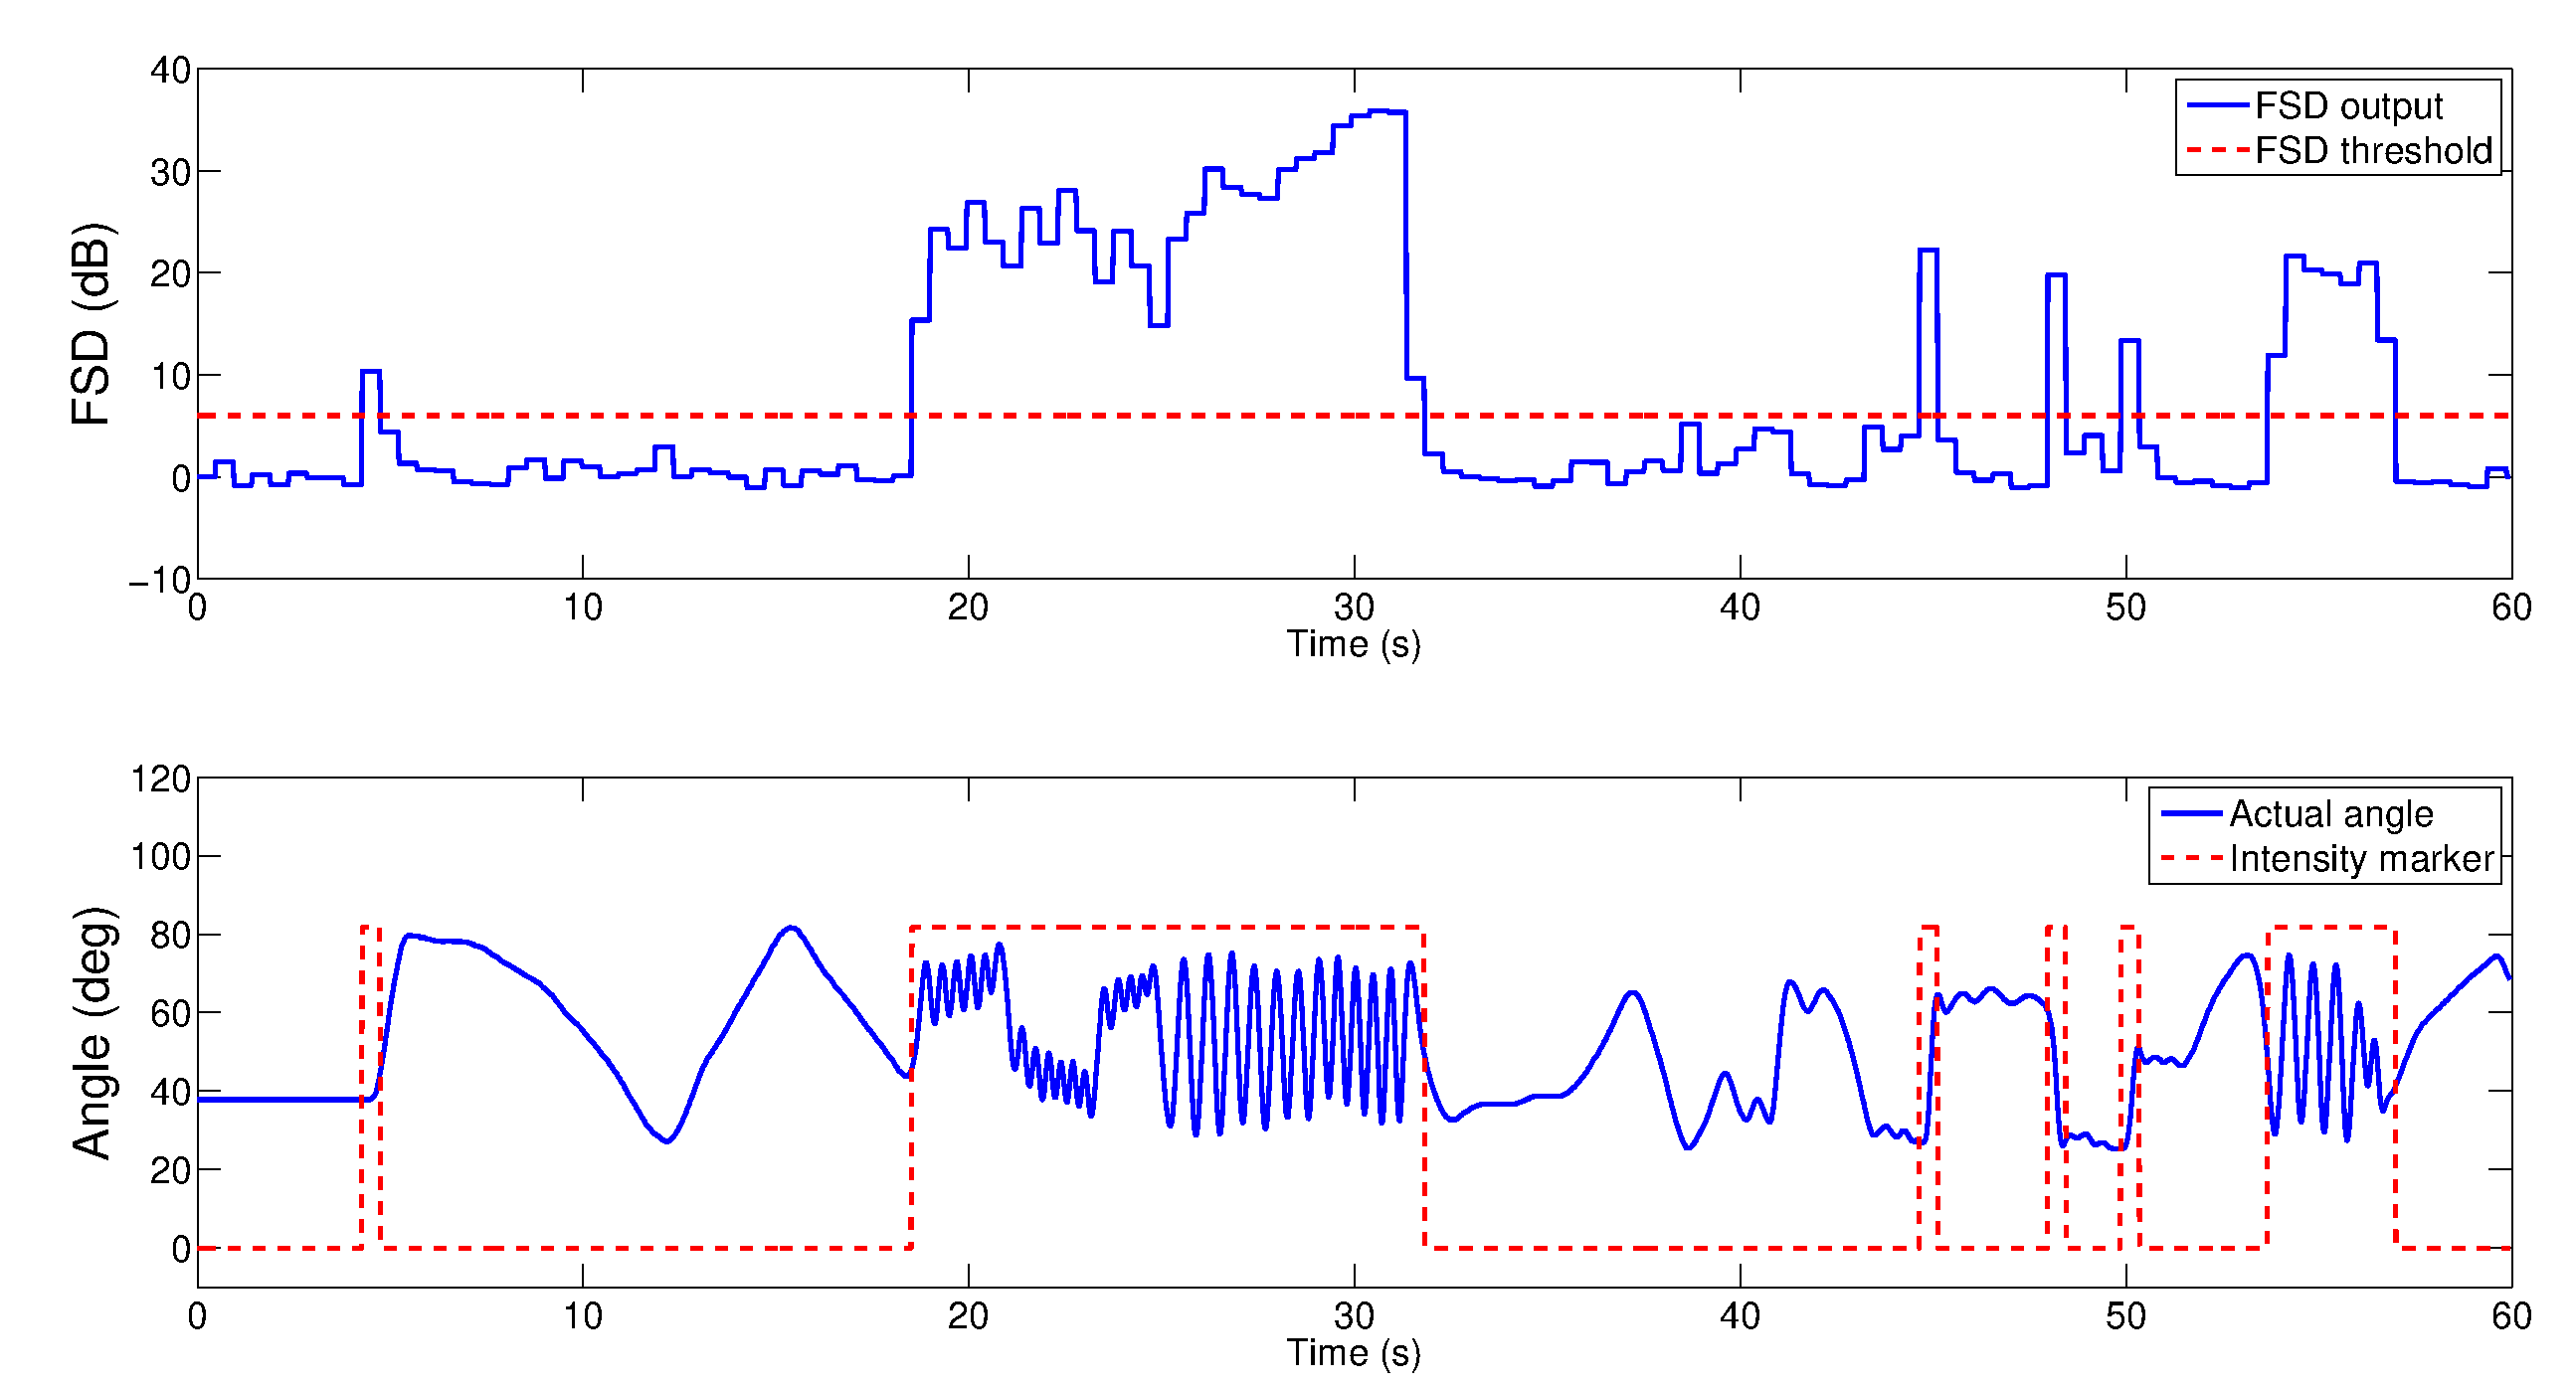
\includegraphics[width=0.88\textwidth]{AAUgraphics/FSD_output.eps}
	\end{column}
\end{columns}

\end{block}
\end{frame}
%%%%%%%%%%%%%%%%%%%%%%%%%%%%%%%%%%%%%%%%%%%%%%%%


%%%%%%%%%%%%%%%%%%%%%%%%%%%%%%%%%%%%%%%%%%%%%%%%
\subsection{Gated Orientation Estimation Algorithms}
\label{subsec:gated_algorithms}
\begin{frame}{Theoretical Background}{Gated Orientation Estimation Algorithms}
\begin{block}{Most orientation estimation algorithms are based on the Kalman filter}
\begin{itemize}
	\item Kalman filter fuses accelerometer, gyroscope and magnetometer data.
	\item Fusion is strictly necessary.
	\item No sensor provides accurate estimates if used individually.
	\begin{itemize}
		\item \textit{Accelerometer} $\rightarrow$ Decomposition of Earth's gravity vector. Only valid if motion is very smooth.
		\item \textit{Gyroscope} $\rightarrow$ Integration of angular rate. Shows large drift.
		\item \textit{Magnetometer} $\rightarrow$ Decomposition of Earth's magnetic field vector. Only valid in magnetically clean environments.
	\end{itemize}
\end{itemize}
\end{block}
\begin{block}{As said before, Kalman filters have constant parameters}
\begin{itemize}
\item Constant covariance matrix of process noise ($Q$).
\item Constant covariance matrix of measurement noise ($R$).
\item We will set 2 different values (intense motion and low motion).
\item The values are changed accordingly (Gating).
\end{itemize}

\end{block}
\end{frame}
%%%%%%%%%%%%%%%%%%%%%%%%%%%%%%%%%%%%%%%%%%%%%%%%


%%%%%%%%%%%%%%%%%%%%%%%%%%%%%%%%%%%%%%%%%%%%%%%%
\begin{frame}{Theoretical Background}{Gated Orientation Estimation Algorithms}
\begin{block}{Structure of the Gated Kalman Filter}
\vspace{0.3cm}
\centering
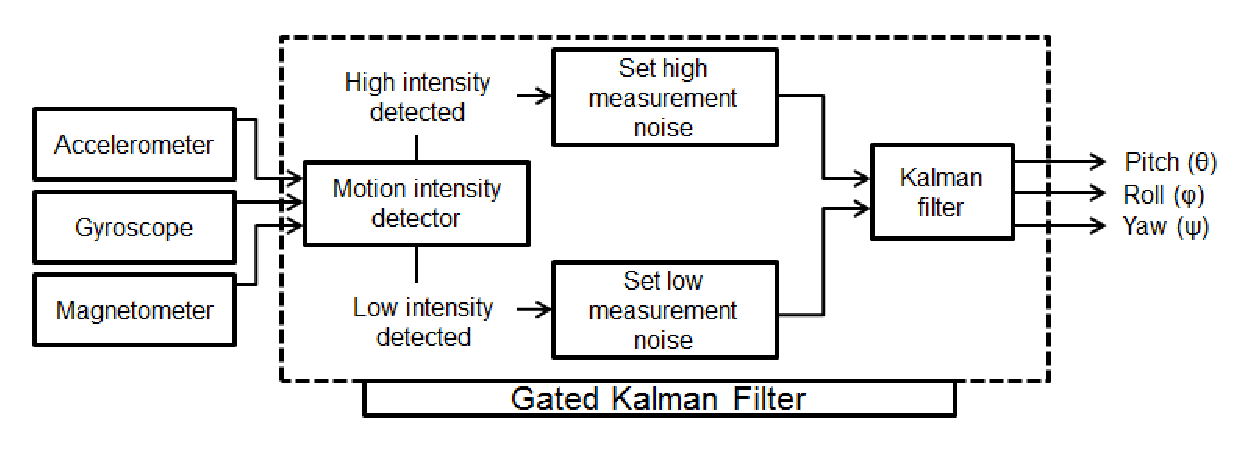
\includegraphics[width=1\textwidth]{AAUgraphics/GKFDiagram.eps}
\begin{itemize}
	\item High intensity $\rightarrow$ high linear acceleration $\rightarrow$ high variance of measurement noise.
	\item Low intensity $\rightarrow$ low linear acceleration $\rightarrow$ low variance of measurement noise.
\end{itemize}
\end{block}
\end{frame}
%%%%%%%%%%%%%%%%%%%%%%%%%%%%%%%%%%%%%%%%%%%%%%%%


%%%%%%%%%%%%%%%%%%%%%%%%%%%%%%%%%%%%%%%%%%%%%%%%
\section{Experiments}
\label{sec:experiments}
\subsection{Experiment Design}
\label{subsec:experiment_design}
\begin{frame}{Experiments}{Experiment Design}
\begin{block}{Datasets}
\begin{itemize}
	\item 16 datasets of inertial and magnetic signals.
	\begin{itemize}
		\item 3D acceleration, 3D angular rate and 3D magnetic field.
	\end{itemize}
	\item MIMU: Wagyromag.
	\item Mechanical device to determine angle reference (ground truth).
	\item Each dataset contains both smooth and intense random motion.
\end{itemize}
\begin{columns}
\begin{column}{.5\textwidth}
\centering
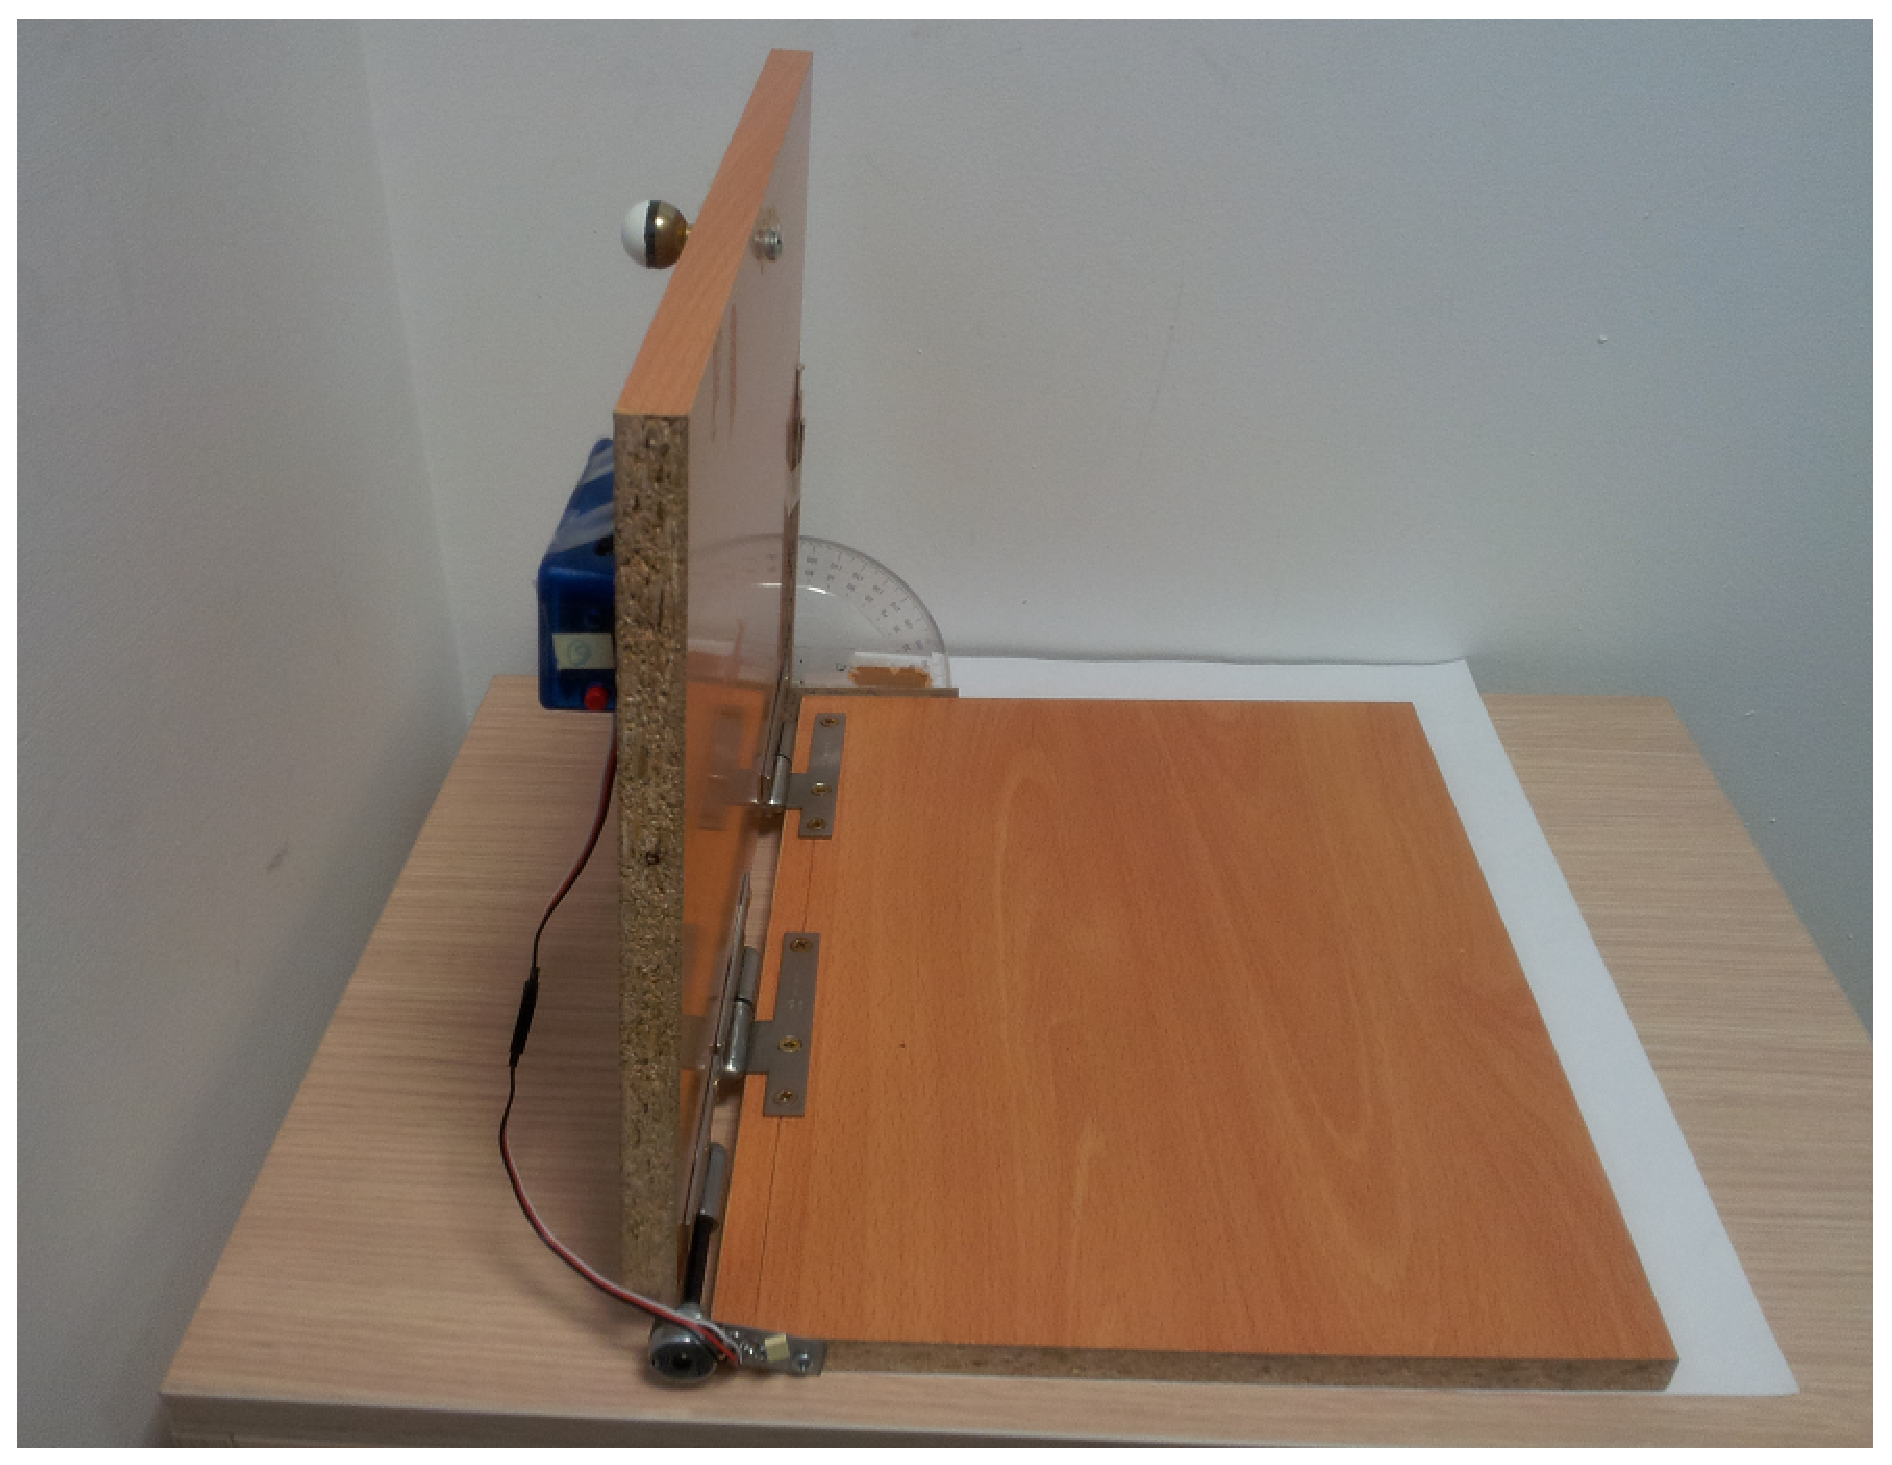
\includegraphics[width=0.85\textwidth]{AAUgraphics/AngleDevice.eps}
\end{column}
\begin{column}{.5\textwidth}
\centering
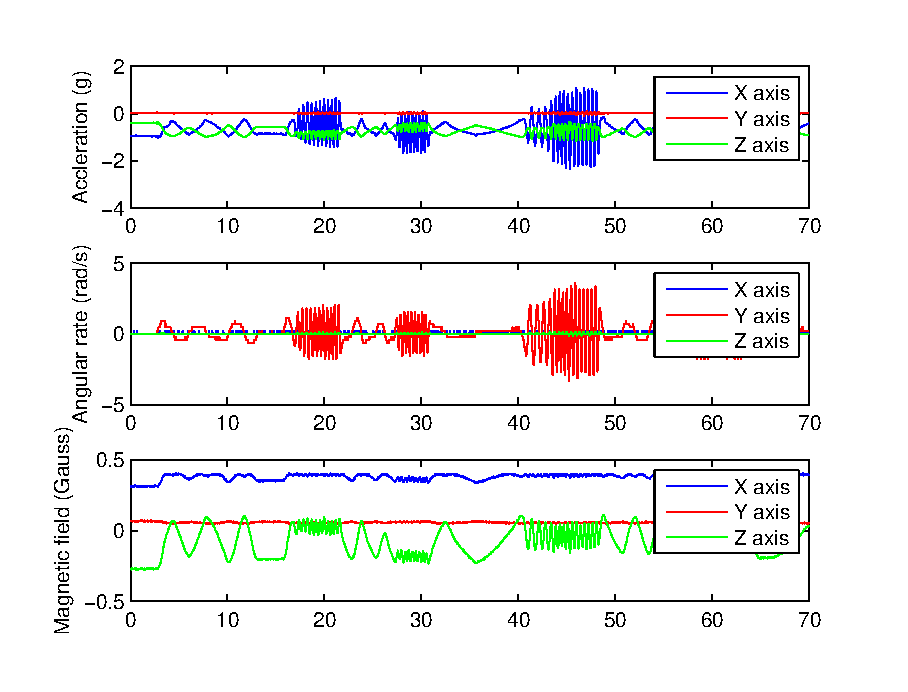
\includegraphics[width=1\textwidth]{AAUgraphics/data_signals.eps}
\end{column}
\end{columns}
\end{block}
\end{frame}
%%%%%%%%%%%%%%%%%%%%%%%%%%%%%%%%%%%%%%%%%%%%%%%%


%%%%%%%%%%%%%%%%%%%%%%%%%%%%%%%%%%%%%%%%%%%%%%%%
\begin{frame}{Experiments}{Experiment Design}
\begin{block}{Algorithms}
\begin{itemize}
	\item 4 orientation estimation algorithms.
	\begin{itemize}
		\item 2 Kalman Filters: QUEST + gyro and gravity decomposition + gyro.
		\item 2 Extended Kalman Filters:  QUEST + gyro and gravity decomposition + gyro.
	\end{itemize}
\end{itemize}
\end{block}
\begin{block}{Experiment Workflow}
We have used a Monte Carlo procedure:
\begin{enumerate}
	\item Load dataset and calibrate signals.
	\item Initialize parameters.
	\item Estimate orientation using all 4 algorithms.
	\item Apply Adaptive Nelder-Mead Simplex Algorithm to minimize RMSE. Optimal parameters are found.
	\item End of loop $\rightarrow$ average RMSE and optimal parameters for each algorithm.
\end{enumerate}
\end{block}
\end{frame}
%%%%%%%%%%%%%%%%%%%%%%%%%%%%%%%%%%%%%%%%%%%%%%%%


%%%%%%%%%%%%%%%%%%%%%%%%%%%%%%%%%%%%%%%%%%%%%%%%
\subsection{Results}
\label{subsec:results}
\begin{frame}{Experiments}{Results}
\begin{table}[t]
\centering
\caption{RMSE of estimated pitch angle with respect to the ground truth. Non-gated vs. gated algorithms. Last row shows the percentage of improvement by using the gated approach.}
\label{tab:results}
\scriptsize
\bgroup
\def\arraystretch{1.3}
\begin{tabular}{ | c | c | c | c | c |}
\hline
					&	\textbf{KF}				&	\textbf{KF (QUEST)}		&	\textbf{EKF}				& 	\textbf{EKF (QUEST)} 	\\\hline
\textbf{RMSE (deg)}			&	$3.00\pm0.72$	&	$1.50\pm0.22$	&	$3.07\pm1.13$	&	$2.26\pm0.48$	\\\hline
					&	\textbf{G-KF}			&	\textbf{G-KF (QUEST)}	&	\textbf{G-EKF}			& 	\textbf{G-EKF (QUEST)} 	\\\hline
\textbf{RMSE (deg)}			&	$2.09\pm0.56$	&	$1.48\pm1.88$	&	$2.35\pm0.97$	&	$2.24\pm0.47$	\\\hline
\textbf{Improvement (\%)} 	&	$\mathbf{\color{orangeUGR}{29.34\pm12.03}}$ &   $0.89\pm5.19$	&	$\mathbf{\color{orangeUGR}{23.31\pm10.70}}$&	$0.93\pm1.77$	\\
\hline
\end{tabular}
\egroup
\end{table}
\centering
\includegraphics[width=0.6\textwidth]{AAUgraphics/angles.eps}
\end{frame}
%%%%%%%%%%%%%%%%%%%%%%%%%%%%%%%%%%%%%%%%%%%%%%%%


%%%%%%%%%%%%%%%%%%%%%%%%%%%%%%%%%%%%%%%%%%%%%%%%
\section{Discussion of Results}
\label{sec:discussion}
\begin{frame}{Discussion of Results}
\begin{block}{Effect of Covariance matrices}
\begin{columns}
\begin{column}{.5\textwidth}
\begin{itemize}
\item Prediction equations:
\end{itemize}

\begin{equation}
\mathbf{\hat{x}}_{k}^{-}=\Phi\mathbf{\hat{x}}_{k-1}
\label{eq:Kal_fus_pred1}
\nonumber
\end{equation}
\begin{equation}
\mbox{P}_{k}^{-}=\Phi\mbox{P}_{k-1}\Phi^{T}+\mbox{Q}
\label{eq:Kal_fus_pred2}
\nonumber
\end{equation}

\begin{itemize}
\item Update equations:
\end{itemize}

\begin{equation}
\mbox{K}_{k}=\frac{\mbox{P}_{k}^{-}\mbox{H}^{T}}{\mbox{H}\mbox{P}_{k}^{-}\mbox{H}^{T}+\mbox{R}}
\label{eq:Kalman_gain_update_phase}
\nonumber
\end{equation}
\begin{equation}
\mathbf{\hat{x}}_{k}=\mathbf{\hat{x}}_{k}^{-}+\mbox{K}_{k}(\mbox{z}_{k}-\mbox{H}\mathbf{\hat{x}}_{k}^{-})
\label{eq:state_vector_update_phase}
\nonumber
\end{equation}
\begin{equation}
\mbox{P}_{k}=(\mbox{I}-\mbox{K}_{k}\mbox{H})\mbox{P}_{k}^{-}
\label{eq:covariance_matrix_update_phase}
\nonumber
\end{equation}
\end{column}
\begin{column}{.5\textwidth}
\begin{itemize}
	\item $\Phi$: state transition matrix.
	\item $\mathbf{\hat{x}}_{k}^{-}$: a priori state estimate.
	\item $\mbox{P}_{k}^{-}$: a priori system covariance matrix.
	\item $\mbox{Q}$: process noise covariance matrix.
	\item R: observation noise covariance matrix.
	\item $\mbox{K}_{k}$: Kalman filter gain.
	\item $\mathbf{\hat{x}}_{k}$: a posteriori state estimate.
	\item $\mbox{P}_{k}$: a posteriori system covariance matrix.
\end{itemize}
\end{column}
\end{columns}
\end{block}
\end{frame}
%%%%%%%%%%%%%%%%%%%%%%%%%%%%%%%%%%%%%%%%%%%%%%%%


%%%%%%%%%%%%%%%%%%%%%%%%%%%%%%%%%%%%%%%%%%%%%%%%
\section{Conclusions and Future Work}
\label{sec:conclusions}
\begin{frame}{Conclusions and Future Work}
\begin{block}{Conclusions}

\begin{itemize}
\item Novel approach to improve precision of determination human body orientation.
\item Applying a gating strategy to Kalman filter.
\item Gating changes formerly permanent parameters according to motion intensity.
\item Motion intensity is detected analyzing spectrum of acceleration magnitude.
\item Experiments show improvement of up to $29\%$ over non-gated approach.
\end{itemize}
\end{block}	
\begin{block}{Future work}
\begin{itemize}
	\item Multi-level variation (instead of 2 intensity levels).
	\item Fuzzy variation of parameters.
\end{itemize}
\end{block}
\end{frame}
%%%%%%%%%%%%%%%%%%%%%%%%%%%%%%%%%%%%%%%%%%%%%%%%

% subsection  (end)
% section conclussions (end)

{\aauwavesbg%
\begin{frame}[plain,noframenumbering]%
  \finalpage{Thank you for your attention!}
\end{frame}}
%%%%%%%%%%%%%%%%

\end{document}
